
%\documentclass{article}

\documentclass[11pt,letterpaper,onecolumn]{article}

\usepackage[english]{babel}
\usepackage[document]{ragged2e}
\usepackage{amsmath}
\usepackage{amsfonts}
\usepackage{graphicx}
\usepackage{ragged2e}
\usepackage[none]{hyphenat}
\usepackage[square]{natbib}
\setcitestyle{super}
\usepackage{url}
\usepackage{amssymb}
\usepackage{xcolor}
\usepackage[bookmarksopen=true]{hyperref}
\usepackage[numbered]{bookmark}
\hypersetup{ pdftitle={Forwarding in Data Center},pdftex, colorlinks=true, citecolor={black}, linkcolor={black}, urlcolor={blue} }
\usepackage{hypcap}


\usepackage[left=1in,right=1in,top=1in,bottom=1in]{geometry}

\def \address{bharat3@ncsu.edu \textbullet \ bharat3 \textbullet \ 200099800}

\makeatletter
\def\@maketitle{%
  \newpage
%  \null% DELETED
 \vskip 0.1em% DELETED
  \begin{center}%
  
  \let \footnote \thanks
    {\LARGE \textbf{\@title} \par}%
    \vskip 0.5em%
    {\large
      \lineskip 0.25em%
      \begin{tabular}[t]{c}%
        \@author\\
       \footnotesize \address
      \end{tabular}\par}%
    \vskip 0.25em%
    {\footnotesize \@date}%
  \end{center}%
  \par
  \vskip 1.5em}
\makeatother

\title{Forwarding in Data Center}
\author{Bharath Ravindranath}

\date {\today}


\begin{document}
{\let\newpage\relax\maketitle}

\section{Introduction}
\justify
\par{\qquad In a data center network with hundreds of thousands of servers or virtual machines serving different tenants, there will be multiple paths to reach a server from core layer. With simple IP protocol each source-destination pair will have a single path. Which will be a bottle neck as we move higher from the edge to core layer of data center. The traditional  destination based routing can be replaced by dynamic routing or policy based routing. Two such proposed solutions are presented in this literature review. One approach uses a two-level routing table to utilize high fan-out available for fat tree topologies\cite{al2008scalable}. Another solution uses a scalable, dynamic flow scheduling system that adaptively schedules a multi-stage switching fabric to efficiently utilize aggregate network resources\cite{al2010hedera}.}
\\

\textbf{\textit{Index terms--} Data Center Network, Scheduling, Forwarding, Policy based routing}

\section{Literature Review}
\justify


\par{\qquad The rest of this literature survey is organized as follows. Section 2.1 gives the details of problems associated with existing scheduling scheme. Sections 2.2 gives a presented solution involving flow based scheduling. Section 2.3 presents <<>>. We conclude the review in Section 3.}


\subsection{Background}

\par{\qquad Data center is a large group of computer servers and storage typically used by organizations for remote storage or processing. Data Center Network (DCN) is critical for the operation since it interconnects the resources of the data center. Also, network architecture needs to be scalable and efficient to accommodate large number of servers. Virtualization adds to the difficulty of design and management \cite{wiki:001}.}\\

\par{Today's data center topologies typically consist of multi-rooted trees. A common architecture involve top of the rack (ToR) switches interconnecting to end of the rack (EOR) switches. Which are in turn connected to core switches. There can be a two, three or multiple levels of switching \cite{wang2015survey}. In these topologies multiple servers are assigned to tenants. The scheduling of servers to a tenant should reduce the bandwidth overhead on all the links of the data center. But most of the existing selection of a path is based on the source/destination pair. Such static scheduling lead to underutilization or over-utilization of some of the links. The traffic in data center can be classified into two major categories: North-South traffic and East-West traffic. North-South traffic is the traffic to/from outside the data center. East-west traffic is the traffic between VMs or servers within the data center. The traffic analysis of data center traffic is limited since the enterprise hosting the data center do not release such data to the public\cite{song2009multi}. We can assume that data intensive applications utilize East-West traffic as well as North-South. Computational applications mostly generate North-South traffic. We can reasonably assume that both N-S and E-W traffic will contribute significantly. Adding to this the virtualization technology makes it difficult for customers to have guarantees that virtualized instances of applications run on the same physical rack. Without this physical locality, applications face inter-rack (North-South) network bottlenecks.\cite{al2010hedera}}\\

\begin{figure}
\centering
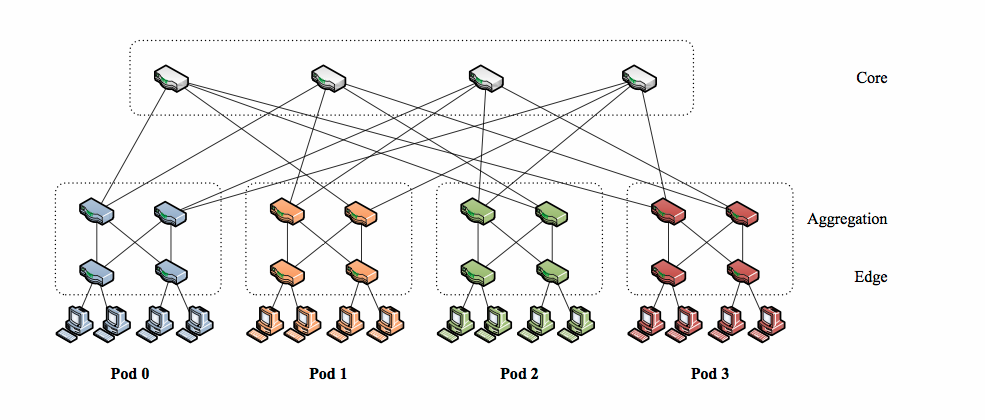
\includegraphics[width=18cm, height=8cm]{fat_tree.png}
\caption{\textit{A three-tired fat tree topology}}
\label{fig:tree}
\end{figure}

\par{A three-tiered architecture is shown in the Figure~\ref{fig:tree}. This is a k-ary fat-tree which contains k pods each with two layers of k/2 switches. Such a design can support approximately 25K hosts. The edge switches will have 1GigE links for host connections and 10GigE for up-link connections. The aggregate and core switchs will have 10GigE or higher links to carry aggregate traffic. We can also use link aggregation to increase the capacity of the links. The ratio of bandwidth at the host level to the bandwidth at the aggregate level is called oversubscription. Oversubscription is the measure of how much traffic the aggregate level can handle in the worst case scenario where all hosts are transmitting at the maximum capacity (1:1 being the best). Typically an oversubscription of 2.5:1 is used in most data centers \cite{al2008scalable}. This type of architecture gives rise two related but different problems. One is the problem of end resource allocation and another is the problem of network resource allocation. Allocating end resources like servers and storage to appropriate tenant is a challenge due to dynamic nature of requests. This type of problem is not taken into consideration in this review. The other problem is of network resource allocation like bandwidth.}\\

\par{From the figure we can see that there are multiple paths we can take from core to edge. The traditional IP protocol cannot use the multipathing feature. The solution should handle loop free multipathing as well as distribute the load among all available paths. Another way of providing a solution is to use policy based routing using deep packet inspection. Deep packet inspection is the packet processing using payload inspection for applications that include contentbased switching like layer-7 switching \cite{dharmapurikar2003deep} \cite{porter2005perils}.}\\

\par{\textit{Policy based routing:} Recently it has become important to select routes in order to restrict the use of network resources to certain classes of customers. These resource policies are not handled adequately by IP routing. For example a network administrator may decide to route packets based on the source address rather than the destination address. Consider the data center topology, if the pod 1 and pod 2 belongs to a single tenant then at the core we cannot make the decision of forwarding based on destination. With destination based routing all the requests from the tenant will be forwarded to only one server. By making the forwarding based on source address we have the ability to say -- ``any request from this tenant is forwarded to either pod1 or pod2". Policy based routing can be based on any of the fields in the packet header or payload like protocol, packet size, etc. To get this information about the required field we use deep packet inspection\cite{wiki:002}. }\\

\par{\textit{Equal cost multi-Path:} Equal-cost multi-path (ECMP) is a routing technique for routing packets along multiple paths of equal cost.  The forwarding engine identifies paths by next-hop.  When forwarding a packet the router must decide which next-hop (path) to use \cite{hopps2000analysis}. The decision could be a hash-map or any other analyzed parameter such as bandwidth requirement of a flow . It can substantially increase bandwidth by load-balancing traffic over multiple paths. Since deep packet inspection is sometimes used to balance the load there may be additional cost involved in processing the packets \cite{wiki:003}.}\\

\subsection{Static routing solution}

\par{\qquad To achieve maximum bi-sectional bandwidth the outgoing traffic from all the pods should be spread evenly among all possible links. In a k-ary fat-tree there will be $(k/2)^2$ shortest paths between any two hosts on different pods. Switches use only one port for traffic going to a particular subnet. The OSPF-ECMP can provide multi-pathing ability. But not all switches have the capability of ECMP  -- its possible and sometimes desirable to have L2 only data centers. Also with multipathing the routing information base increases drastically at lower level switches. A simpler solution is provided by ``A Scalable, Commodity Data Center Network Architecture"\cite{al2008scalable}.}\\

\par{\textit{Addressing:} Assume that all the subnets of the data center have a common prefix i.e. it is subneted from a single network address. This is a reasonable assumption due to the availability of class A private addresses. This can accommodate approximately $2^24$ hosts.}\\

\par{\textit{Two level routing table:} The paper \cite{al2008scalable} provides an implementation of two-level prefix lookup. An entry in the routing table may have a pointer to another secondary routing table entry. The first table will be a prefix based table as in the classic IPv4 routing table i.e. a /m prefix mask, masks the last first m bits by making the last $32-m$ bits as $0$. The secondary table is a suffix table where a /m mask will mask the last m bits by making first $32 - m$ bits as $0$. The routing table entry is said to be terminating if there are no second level suffixes. The secondary table can point to more than on first-level entry. This will not make use of multi-pathing for a single source/destination pair. The following example illustrates the use of two level routing.}\\

\par{ Consider that the two servers in Pod 1 have the IP address 10.1.0.2 and 10.1.0.3 which are connected to the same edge switch. The server 10.1.0.2 is communicating with a server 10.5.1.2 on Pod 3 and server 10.1.0.3 is with a server 10.5.1.3  in the same Pod 3. With traditional IP forwarding we will have one routing table entry for the prefix 10.5.0.0/16 at the edge switch and hence both these requests take the same route. With two-level routing we will have a secondary table for the prefix 10.5.0.0/16. In this secondary table we will have different outgoing ports for different ``suffix" i.e. for 0.0.0.2/16 and 0.0.0.3/16 we make the edge switch to take different aggregate switches. Hence both requests take different paths to the same subnet (10.5.0.0). Although there is a small overhead added to the routing table lookup, the paper argues that the addition is worth paying to achieve traffic fan out.}\\

\subsection{Dynamic scheduling solution}
\par{\qquad A static scheduling will only consider the distribution of routes among all possible paths. But it does not take into account the amount of traffic generated by individual hosts. It is quite possible that some of the servers generate continuous high amount of traffic compared to others. Hence we will need dynamic approach to overcome this backlog. Two such alternatives are discussed in this review: Local flow classification and Centralized flow scheduling}\\

\subsubsection{Local Flow Classification}
\par{ \qquad As an alternate we can perform flow classification with dynamic port-reassignment. We can avoid local congestion in pod switches. Here if there is contention for same output port another port of the same cost is assigned if such a port exists. Flow is defined as the certain set of fields in the packet header. For example set of source address, destination address and destination port number can be defined as a flow. Once we define the flow we have to assign a flow to some outgoing interface. Subsequent packets in the same flow should take the same outgoing interface. But this is local to each switch so its possible that a particular switch is overloaded while others are under-utilized.}\\


\subsubsection{Central Flow scheduling}
\par{\qquad In this approach we use a central scheduler. Each switch in a data center is typically connected to a management switch. This management switch can act as the central scheduler. An OpenFlow switch using SDN is one of the options. This scheduler modifies the forwarding table of the edge and aggregation switches dynamically based on updates from the data center network. The scheduler assigns the flows so as to minimize overhead and spread the resource utilization evenly across the data center.}\\

\par{The scheduler keeps track of the flows. If the flow is small it takes the default static route. If the flow persists for some time and bandwidth requirements reach a threshold , a path is assigned to it. Based on this assigned path the scheduler modifies the routing entries in edge and aggregation switches. Once the flow terminates the flow entries also expire after a certain amount time.}\\

\subsection{Example data center setup}
\par{\qquad Considering the above fat tree topology, we can configure the data center as follows to achieve the above optimizations. First run OSPF-ECMP as the routing protocol between the core and edge switches. This will facilitate the East-West traffic between the servers. The core switches are usually connected to a gateway. At the gateway we can implement the firewall to only permit traffic belonging to relevant tenants. This can be done using policy based routing. Then we create a GRP tunnels between the core and the edge switches. At the core each tenant is identified and appropriate tunnel is used to reach the tenants server\cite{headquarters2007cisco}. The tenant identification can be a policy based routing as well using access control lists (ASL). The mapping of tenants to a GRE tunnel can be automated using BGP configuration. We configure each edge switch into different BGP ASs and the core into another AS. This way we can control the route advertisement sent by servers and the core switches. This helps in keeping the forwarding table small. We can deploy a management switch which connects all the switches in the data center. For example an OpenFlow switch. This is the centralized control for dynamic flow based scheduling. Here we get the analysis results from all the switches and decide which links are overloaded and which are not. Each time we get a flow to be scheduled the controller decides which route to take and then inform all the intermediate switches about this path and flow. This way we can fan out all the requests among all available links. }\\


\section{Conclusion}



\RaggedRight
\newpage
\bibliography{biblio}
\addcontentsline{toc}{section}{\refname}
\bibliographystyle{unsrt}



\end{document}